% vim: set spell spl=cs:
\documentclass[aspectratio=169]{beamer}
\usetheme{einfra2}

\usepackage[utf8]{inputenc}
\usepackage[czech]{babel}

\title{Predikce hmotnostního spektra neuronovými sítěmi}
\author{Filip Jozefov, Adam Hájek, Aleš~Křenek}
\date{Sitsem, 14.9.2023, Telč}

\begin{document}
\makeatletter
\maketitle

\begin{frame}
{Cesta tam}{\dots a ještě ne zpátky}

\begin{itemize}
\item Známe vzorec molekuly, zpravidla jako tzv.\ SMILES: \qquad
\vbox to0pt{
\hsize=1em

\includegraphics[height=12ex]{thc-formula}
\par
\vss
}

\medskip
CCCCCc1cc(c2c(c1)OC([C@H]3[C@H]2C=C(CC3)C)(C)C)O 


\medskip
\pause
\item Chceme predikovat hmotnostní spektrum této látky 

\medskip
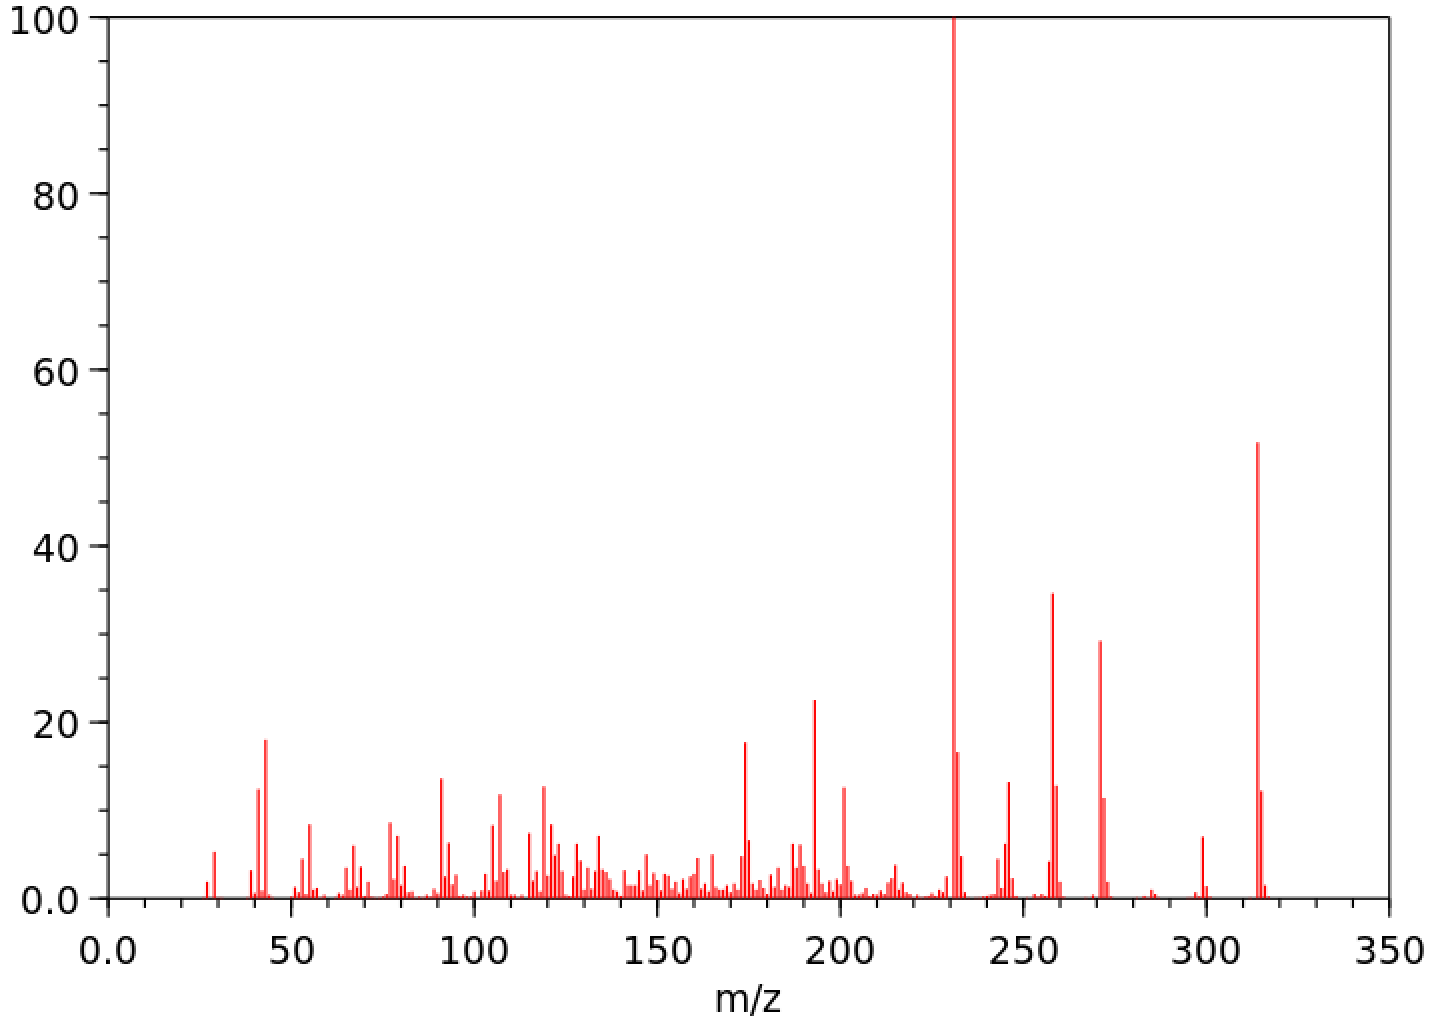
\includegraphics[width=.4\hsize]{thc-spec}
\end{itemize}
\end{frame}

\begin{frame}
{Možné přístupy}
\begin{itemize}
\item \emph{Ab initio} -- kvantově-chemická simulace dějů při štěpení molekuly
\begin{itemize}
\item potenciálně nejpřesnější
\item výpočetní náročností neúnosné (dny až týdny výpočtu pro jednu molekulu)
\end{itemize}
\medskip
\item Empirické -- založené na expertních pravidlech štěpení vazeb atd.
\begin{itemize}
\item nepřesné, omezená doména
\end{itemize}
\medskip
\item \textbf{Strojové učení} na základě desítek až stovek tisíc příkladů
\begin{itemize}
\item neuronové sítě, inspirace jazykovými modely
\item uspokojivá rychlost i přesnost, ale stále je co dělat
\end{itemize}
\end{itemize}
\end{frame}

\begin{frame}
{Známé a neznámé cesty}
\begin{itemize}
\item NEIMS -- Neural Electron-Ionization Mass Spectrometry
\begin{itemize}
\item J.~N.~Wei et.~al, 2019, \url{http://doi.org/10.1021/acscentsci.9b00085}
\item jednoduché, rychlé, robustní, nepříliš přesné
\end{itemize}
\medskip
\item RASSP -- Rapid Approximate Subset-Based Spectra Prediction 
\begin{itemize}
\item R.~L.~Zhu, E.~Jonas, 2023, \url{http://doi.org/10.1021/acs.analchem.2c02093}
\item komplexní zachycení struktury, výrazně přesnější, možnost vysokého rozlišení
% \item omezená velikost a složitost molekuly, výrazně pomalejší
\end{itemize}
\medskip\pause
\item Bonus na cenu děkana
\begin{itemize}
\item tři vlastní řešení, grafové NN a transformery
\item robustní, rychlá a přesnější než NEIMS, bez omezení RASSPu
\end{itemize}


\end{itemize}
\end{frame}

\begin{frame}
{NEIMS}{\dots jednodušší už to být nemůže}
\begin{itemize}
\item Molekula popsána systémem \emph{fingerprintu}
\begin{itemize}
\item konkrétně délky 4096 bitů, ,,1`` znamená výskyt specifické podstruktury
\item standardizovaný postup výpočtu
\end{itemize}
\item Spektrum kódováno přímočaře jako vektor
\begin{itemize}
\item jedna složka pro každou celočíselnou hodnotu $m/z$
\end{itemize}
\end{itemize}
\end{frame}

\begin{frame}
{NEIMS}
\begin{itemize}
\item Jednoduchá architektura neuronové sítě
\begin{itemize}
\item MLP, 7 skrytých vrstev po 2000 neuronech
\item ReLU, dropout 25\,\%
\end{itemize}
\item Zdvojená poslední vrstva
\begin{itemize}
\item fingerprinty vystihují lépe malé fragmenty, model je přesnější pro malá $m/z$
\item přidána tzv. \emph{reverzní predikce}, počítá špičky $M-m/z$ z~téže předposlední vrstvy
\item vrací zpět informaci o celkové hmotnosti $M$
\end{itemize}
\item Loss funkce -- hmotností vážená MSP (obdoba $\textbf{DP}_{1,0.5}$)
\end{itemize}
\end{frame}

\begin{frame}
{NEIMS}
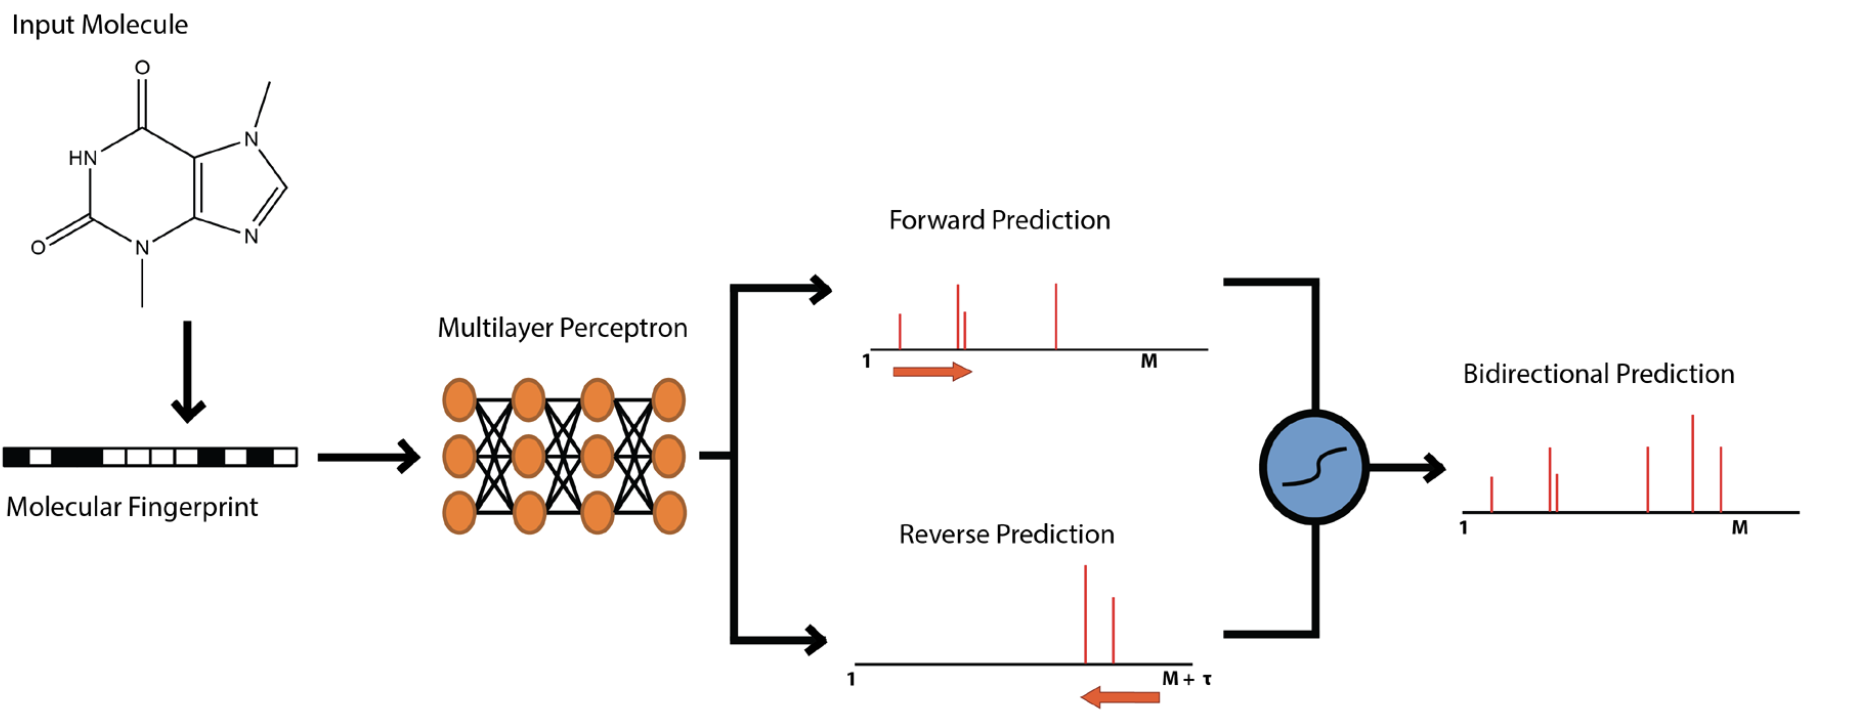
\includegraphics[width=\hsize]{neims.png}
\end{frame}

\begin{frame}
{NEIMS -- výsledky}
\begin{itemize}
\item Společná trénovací (113k) a testovací (28k) sada pro všechny modely 
\item $\textbf{DP} = 0.832\pm0.108, \textbf{SDP}=0.828\pm 0.136$ na testovací sadě
\end{itemize}
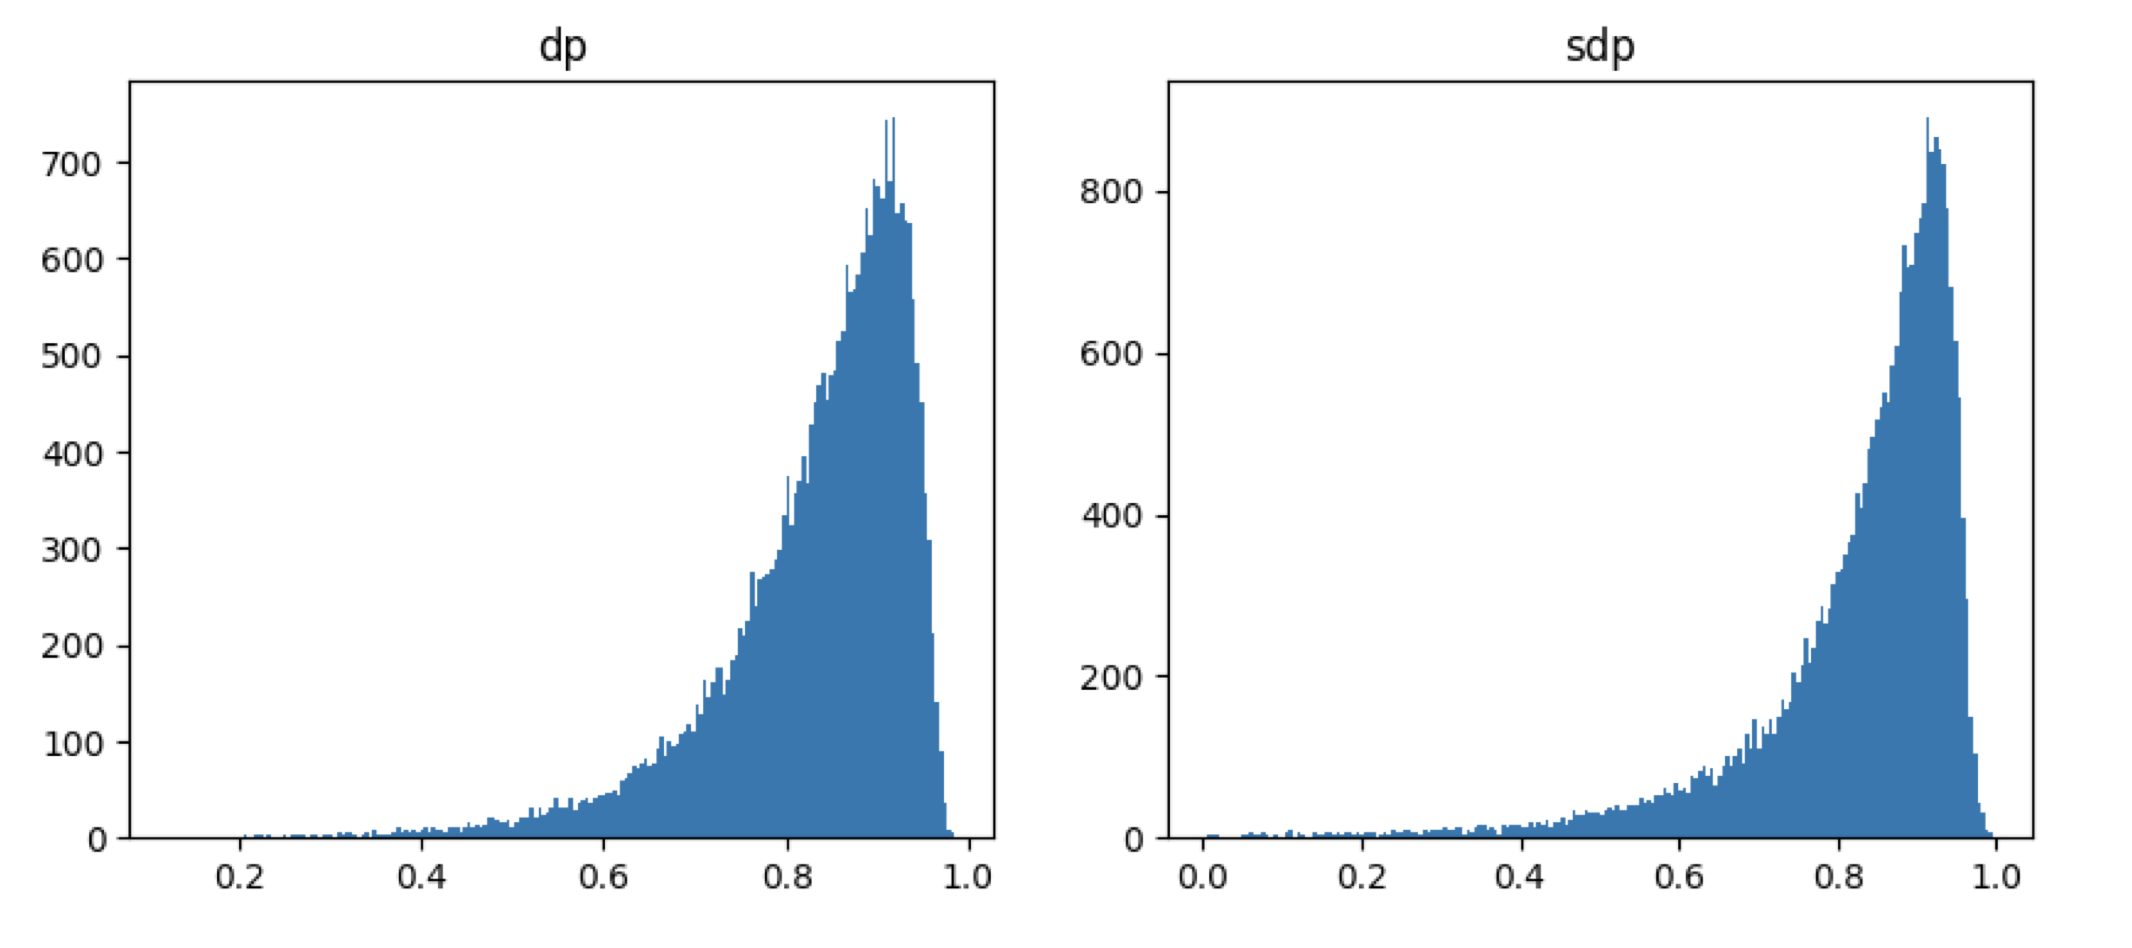
\includegraphics[width=.6\hsize]{neims-hist}
\end{frame}

\begin{frame}
{NEIMS -- výsledky}
\begin{itemize}
\item Nepovedená predikce $\textbf{DP} = 0.41$
\end{itemize}
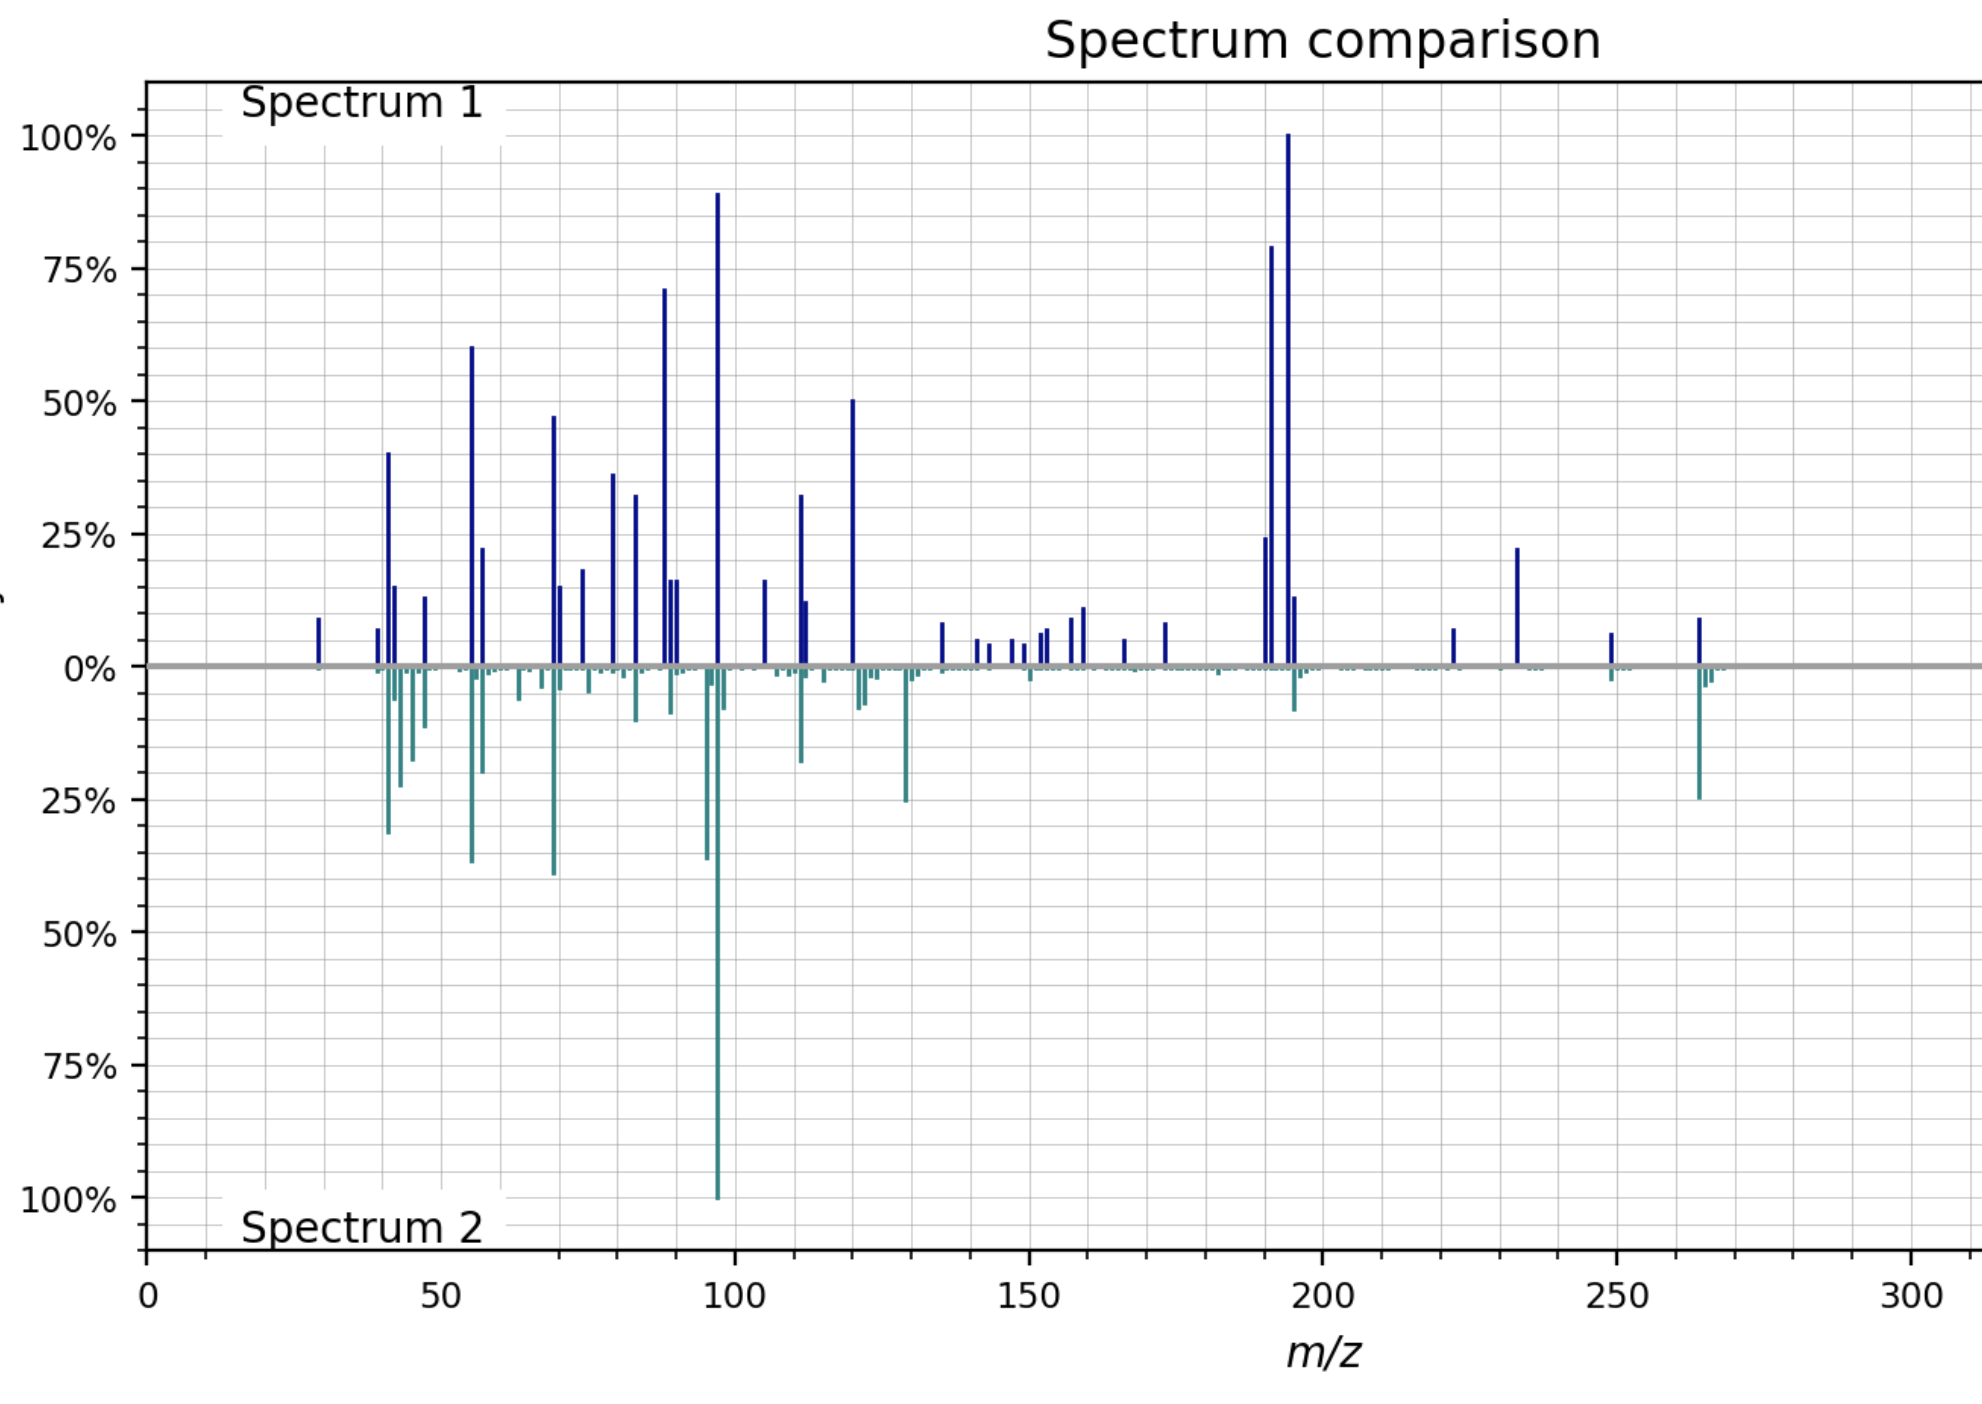
\includegraphics[width=.6\hsize]{compare_041}
\end{frame}

\begin{frame}
{NEIMS -- výsledky}
\begin{itemize}
\item Průměrná predikce $\textbf{DP} = 0.76$
\end{itemize}
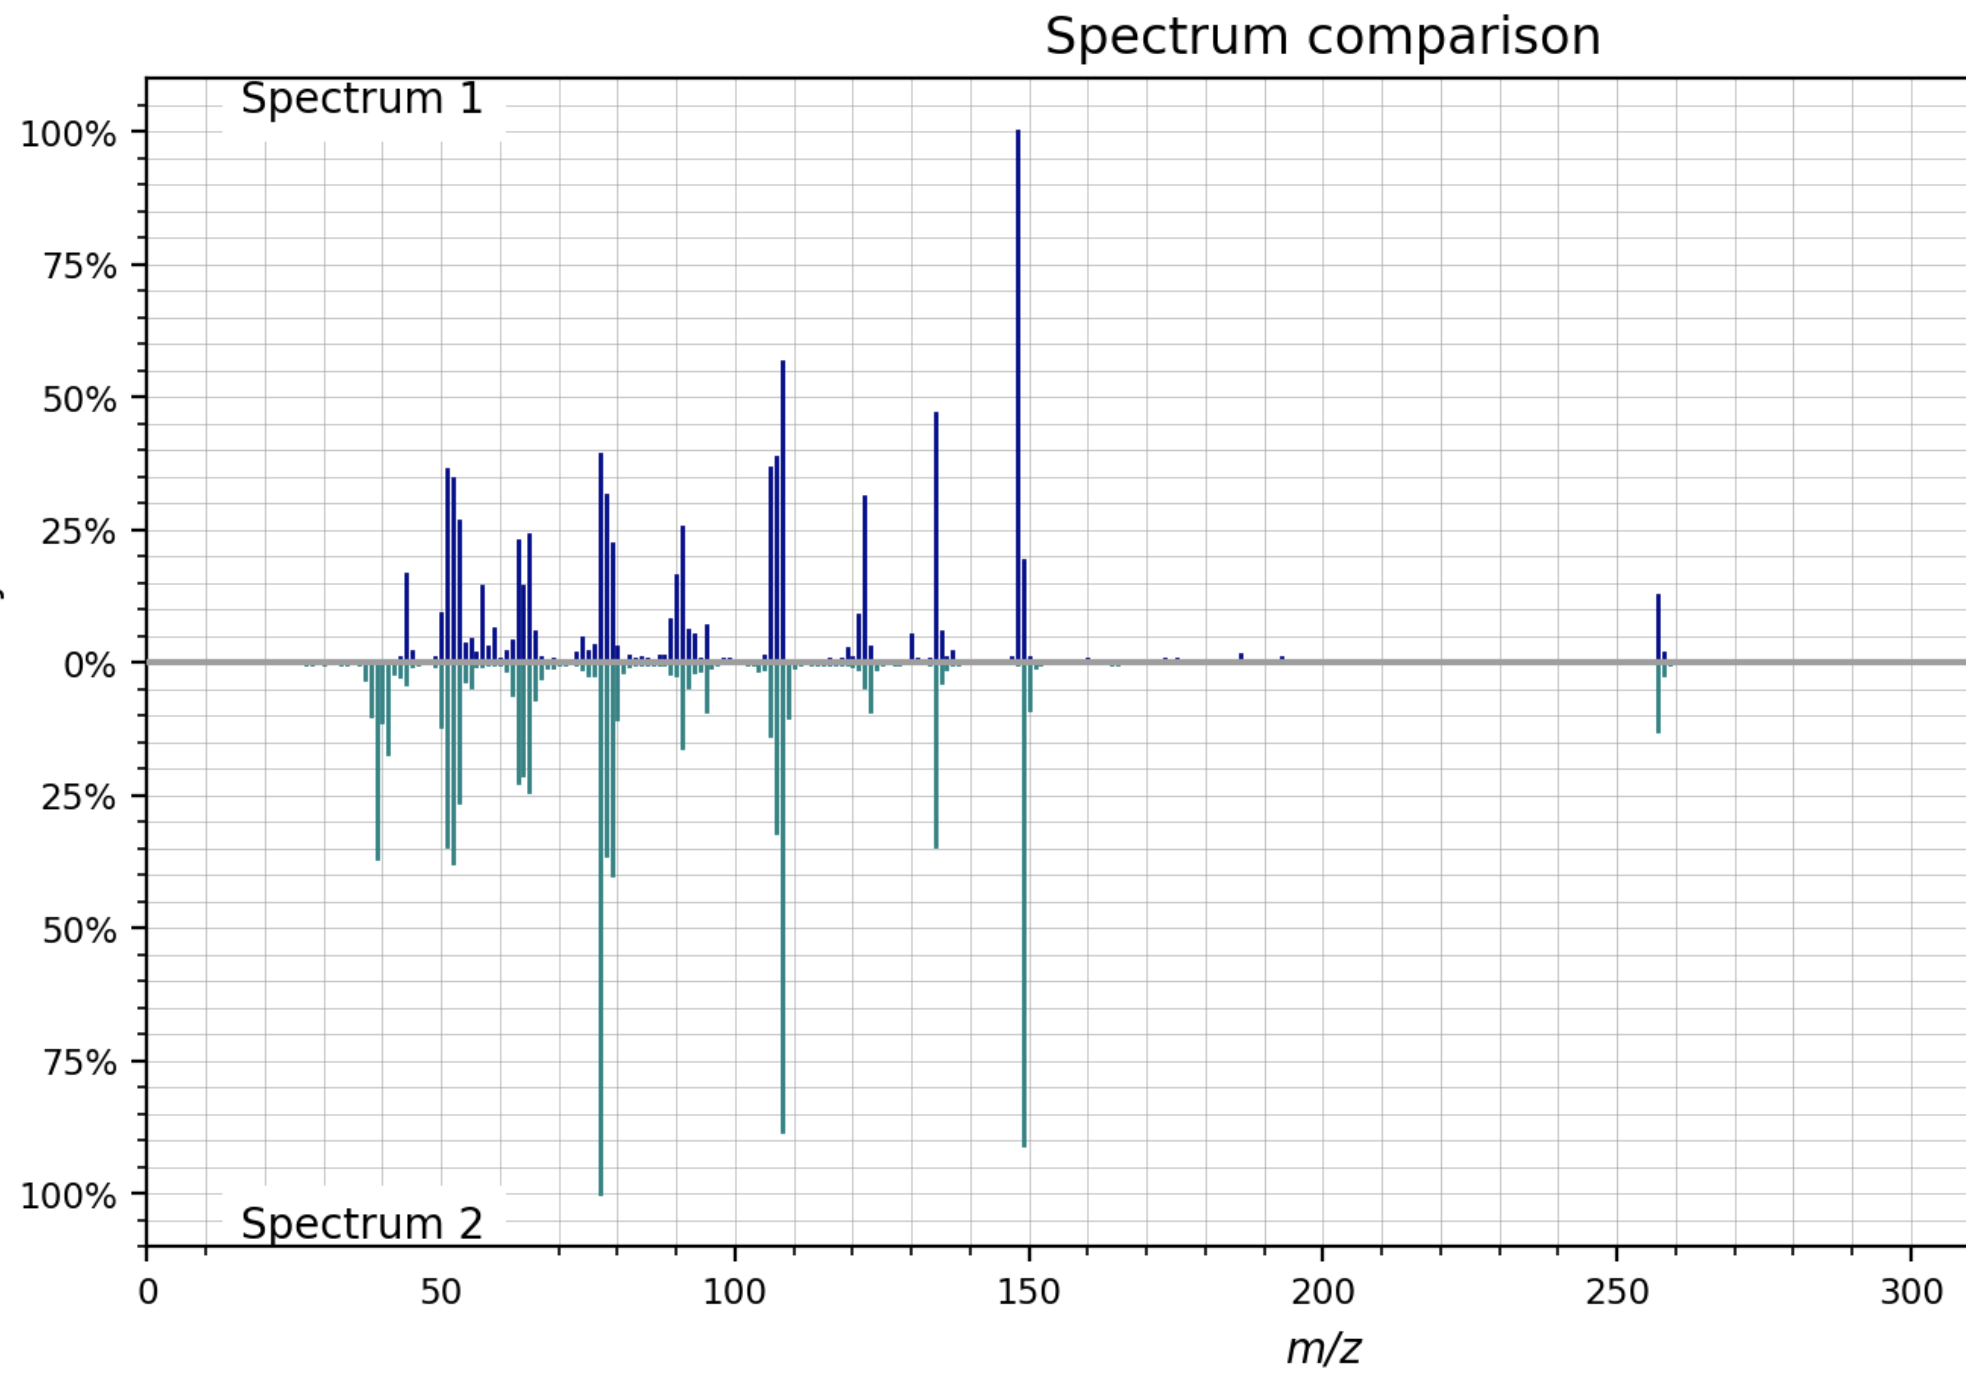
\includegraphics[width=.6\hsize]{compare_076}
\end{frame}


\begin{frame}
{NEIMS -- výsledky}
\begin{itemize}
\item Úspěšná predikce $\textbf{DP} = 0.97$
\end{itemize}
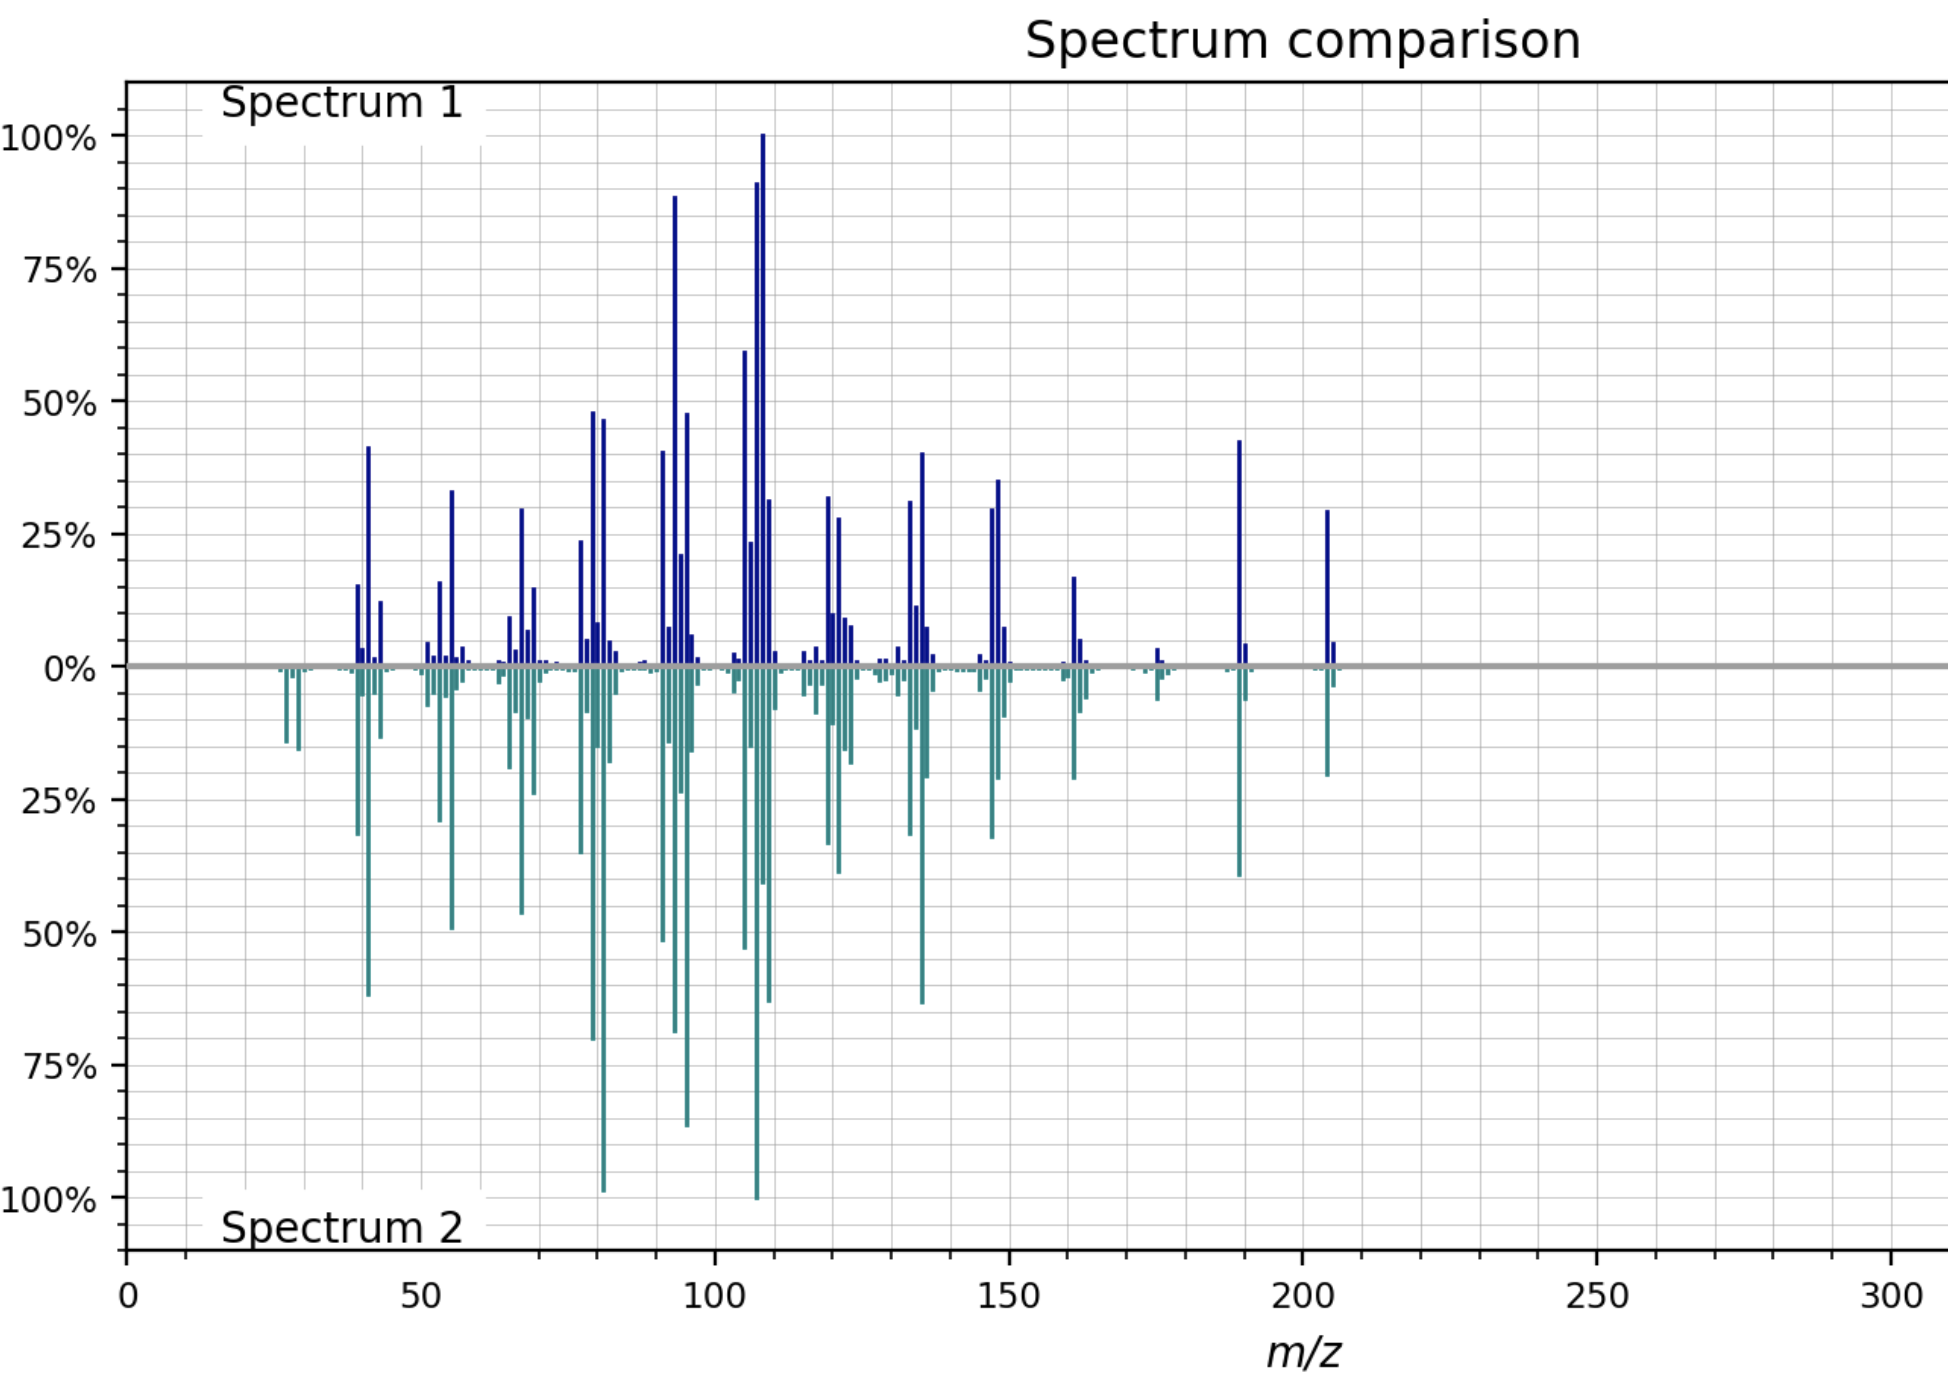
\includegraphics[width=.6\hsize]{compare_097}
\end{frame}



\begin{frame}
{NEIMS -- výsledky}
\begin{itemize} 
\item[$+$] rychlost tréningu i inference
\item[$+$] bez omezení struktury a velikosti molekuly
\item[$-$] pro naše účely nedostatečná přesnost
\item[$-$] nerealisticky ,,chlupatá`` výstupní spektra
\end{itemize}
\end{frame}

\begin{frame}
{RASSP}{\dots složitěji to nevymyslíme}

\begin{itemize}
\item Trénovaný model fragmentace
\begin{itemize}
\item vstup: přímo zakódovaná struktura 
\item výstup: pravděpodobnost výskytu všech sumárních podformulí  \\
(pro vodu H, H$_2$, O, OH, H$_2$O)
\end{itemize}
\item Výpočet spektra z pravděpodobností podformulí
\begin{itemize}
\item deterministicky dán hmotností atomů
\item snadno rozšiřitelný o izotopy
\item možnost vysokého rozlišení v $m/z$ \\
(CH$_4\sim{}$16.043 vs.\ O${}\sim{}$15.999)
\end{itemize}
\end{itemize}
\end{frame}

\begin{frame}
{RASSP}
\begin{itemize}
\item Kódování vlastností atomů (feature embedding)
\begin{itemize}
\item 10 jednoduchých charakteristik atomu (prvek, počet vazeb, typ orbitalu, \dots) \\
celkem 45 numerických parametrů (one-hot kódování)
\item atomy -- vrcholy grafu, vazby -- hrany $\rightarrow$ grafová neuronová síť\\
(16 vrstev \`a 512${}\times{}$512 parametrů)
\item postihuje vlastnosti atomů i jejich vztahy na větší vzdálenost (cf.~fingerprint)
\end{itemize}
\pause
\item Kódování podformulí
\begin{itemize}
\item pouze 8 přípustných typů atomů
\item počty omezeny na 30--50 (podle typu)
\item kumulativní one-hot vektor
\item pro daný vstup se vygenerují všechny
\end{itemize}
% \item Loss funkce -- modifikovaná MSE na spektrech (obdobně NEIMSu)
\end{itemize}
\end{frame}

\begin{frame}
{RASSP}
\begin{itemize}
\item Promíchat, netřepat -- attention + softmax $\rightarrow$ pravděpodobnosti fragmentů
\end{itemize}
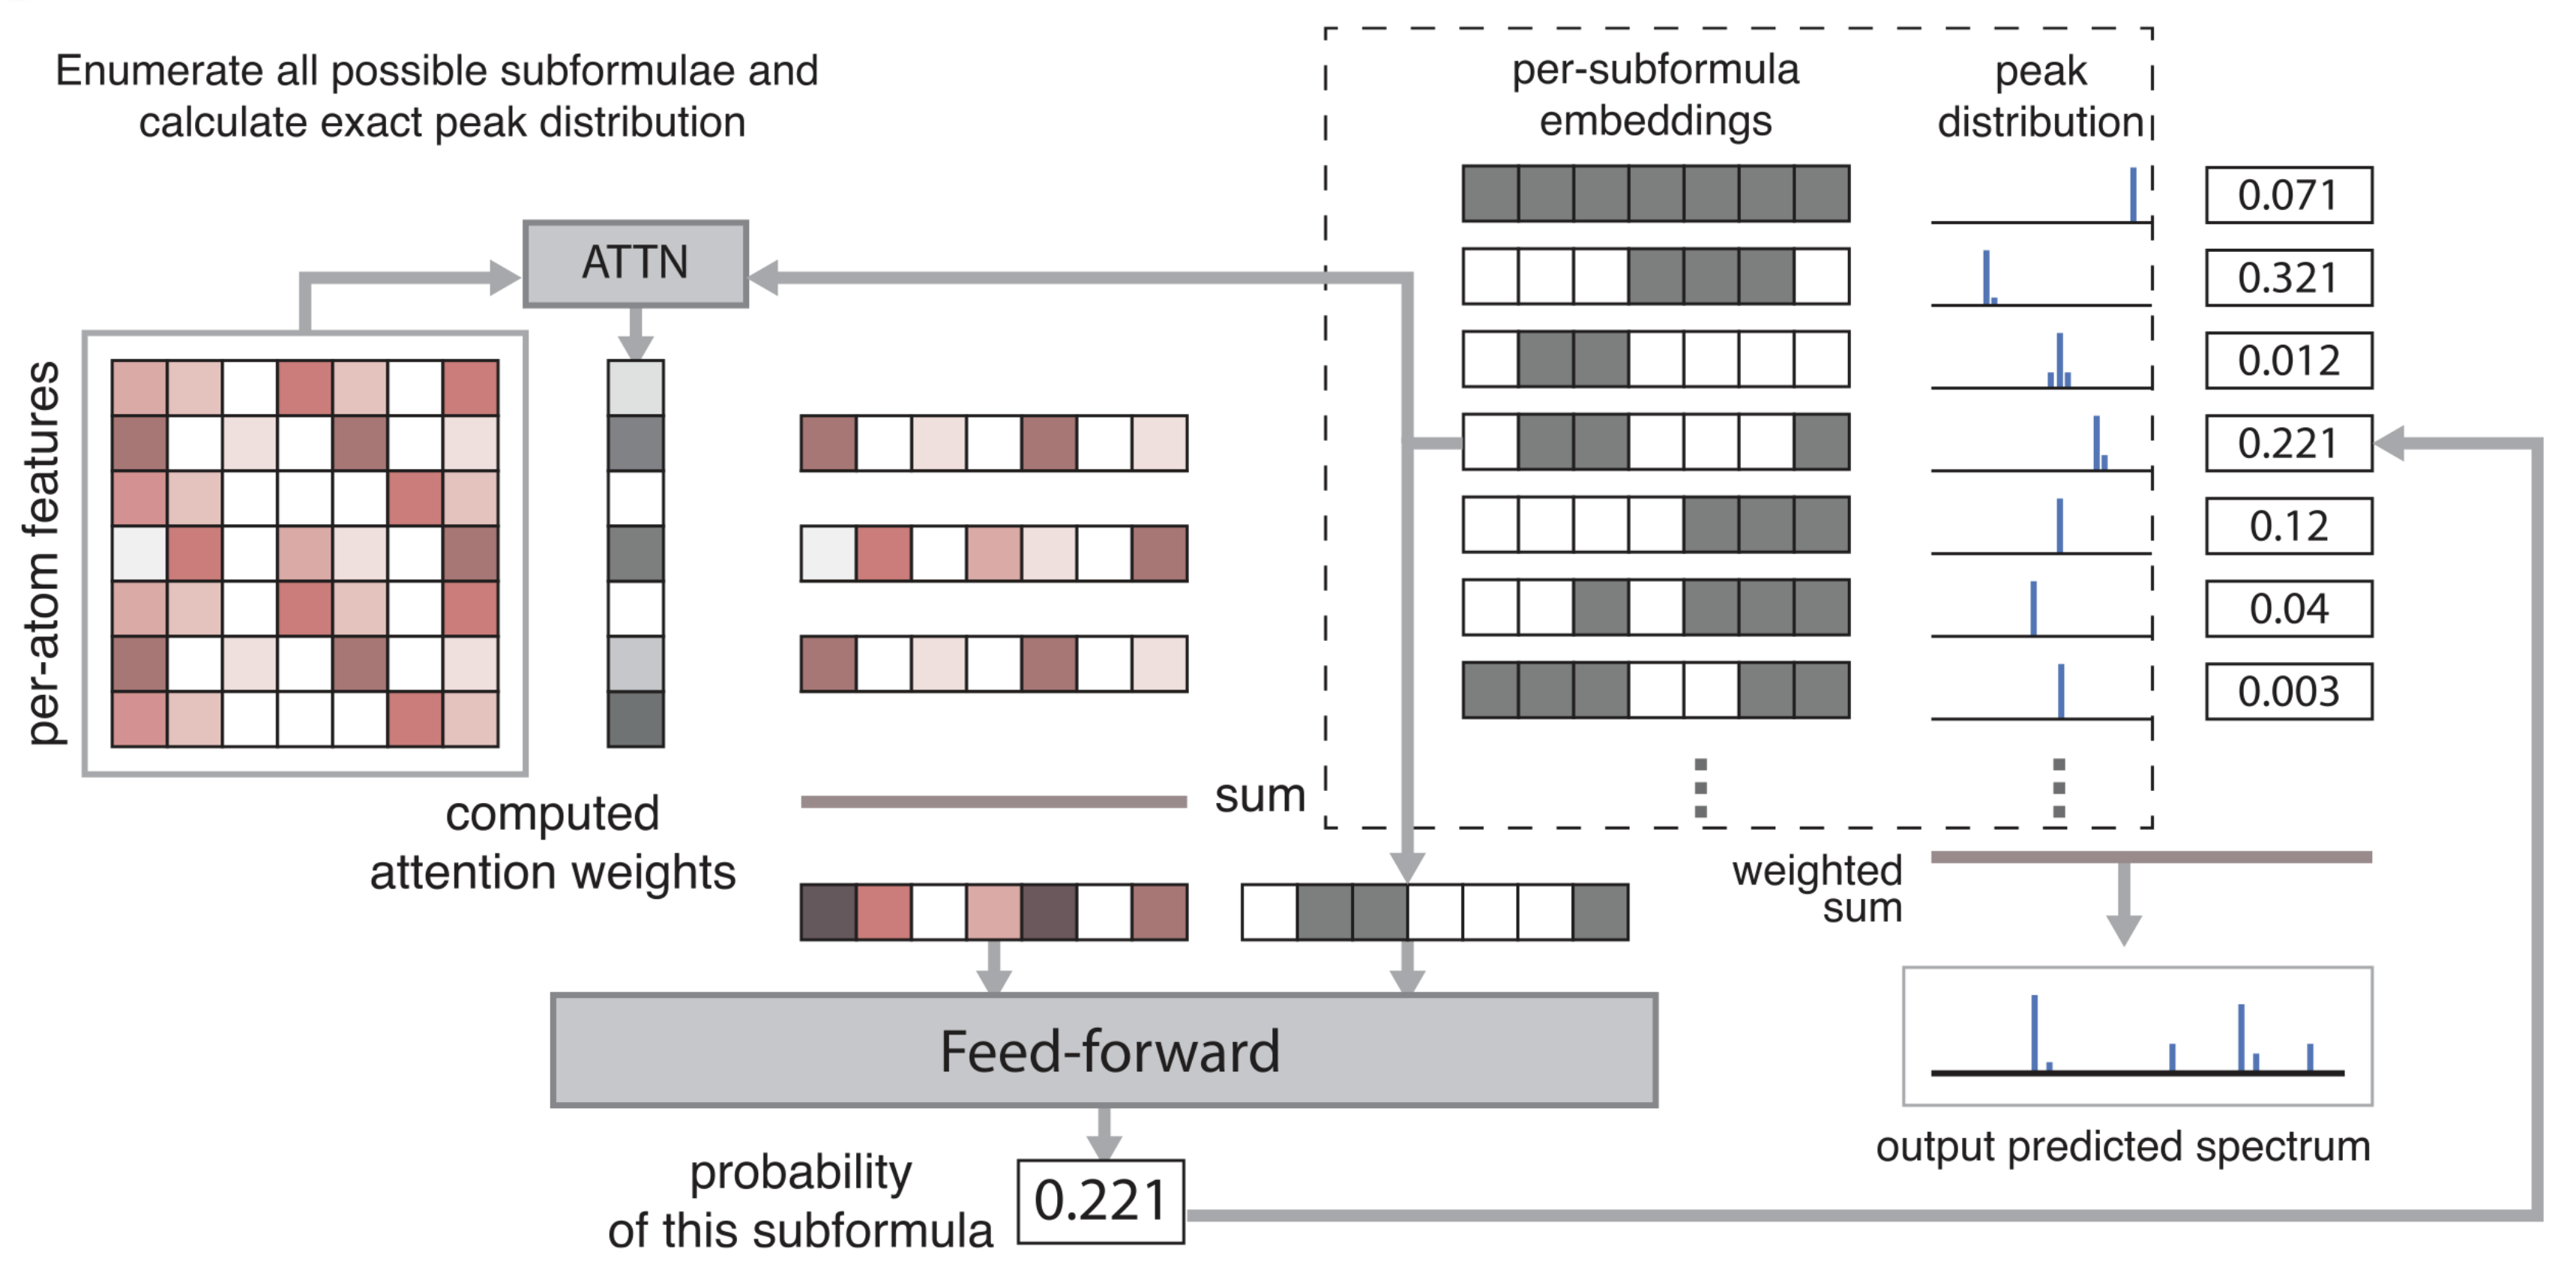
\includegraphics[width=.9\hsize]{rassp-arch}
\end{frame}

\begin{frame}
{RASSP -- výsledky}
\begin{itemize}
\item RASSP: $\textbf{DP}= 0.886\pm0.110, \textbf{SDP}=0.882\pm0.158$
\item NEIMS: $\textbf{DP} = 0.832\pm0.108, \textbf{SDP}=0.828\pm 0.136$ 
\end{itemize}
%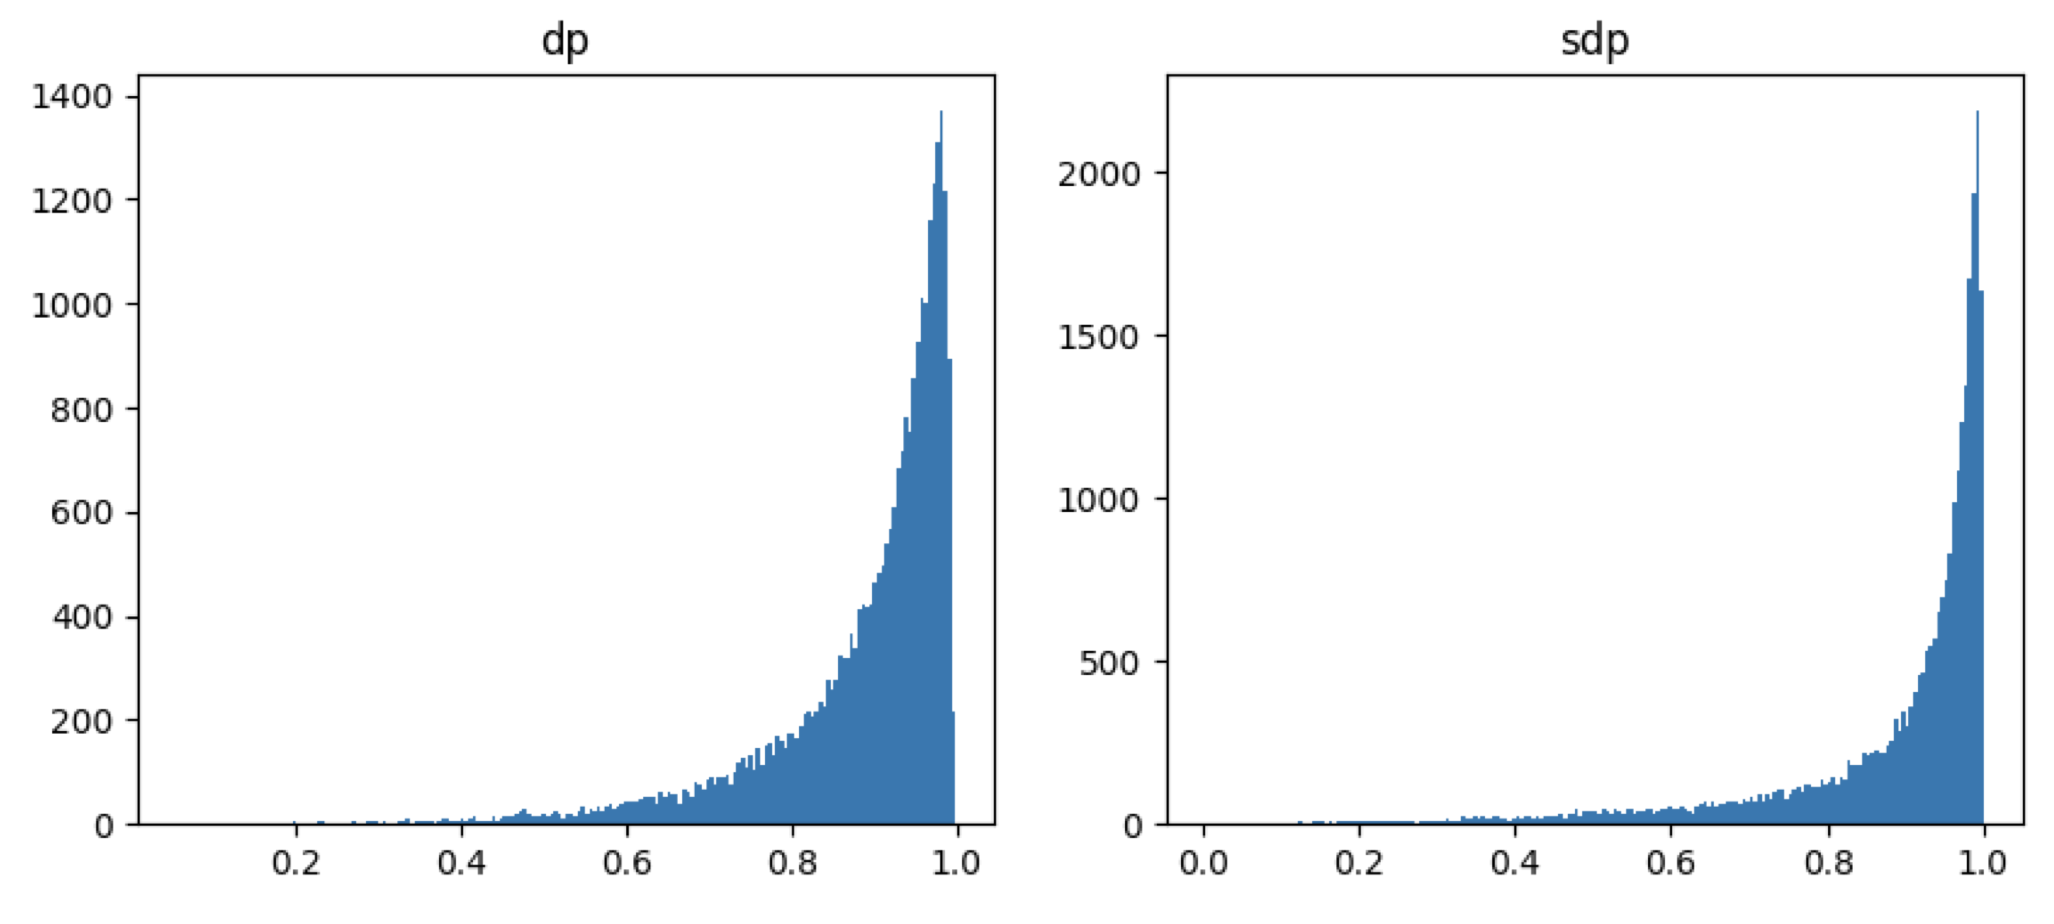
\includegraphics[width=.6\hsize]{rassp-hist}
%\end{frame}
%
%\begin{frame}
%{RASSP -- výsledky}
\begin{tabular}{ll}
\raise3ex\hbox{RASSP} & 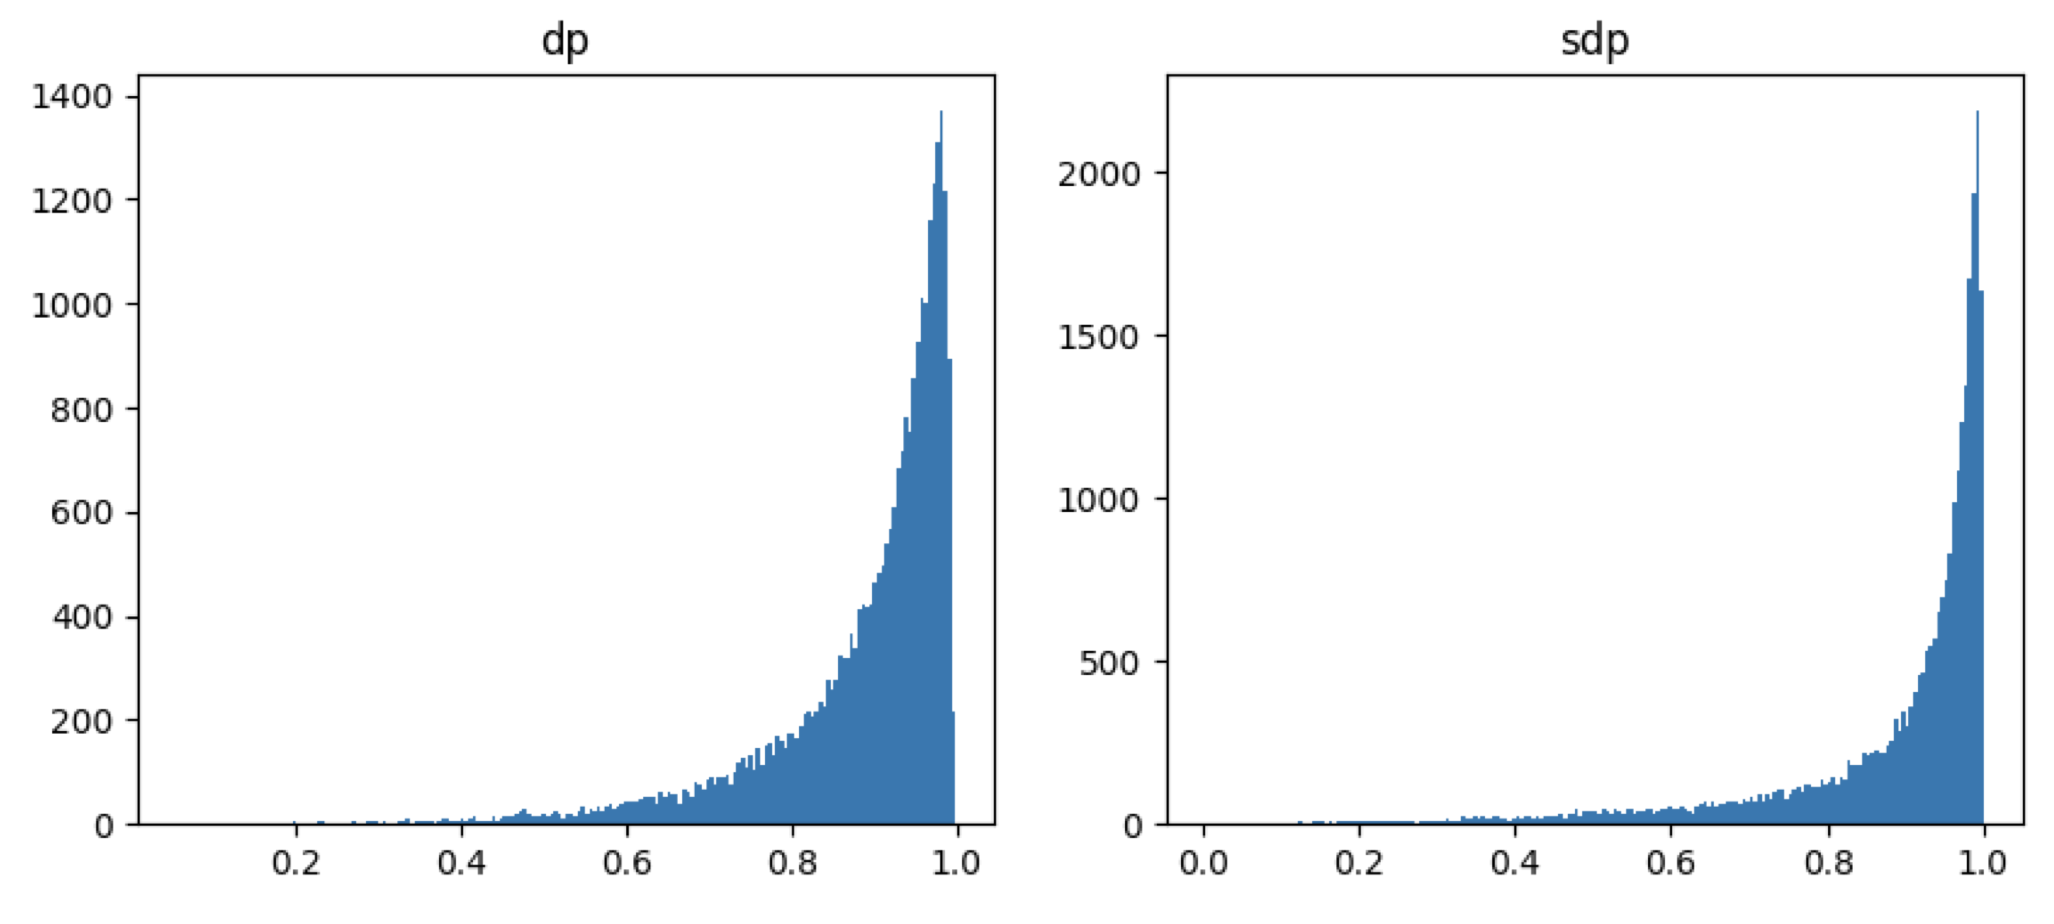
\includegraphics[width=.8\hsize,height=.15\hsize]{rassp-hist} \\
\raise3ex\hbox{NEIMS} & \,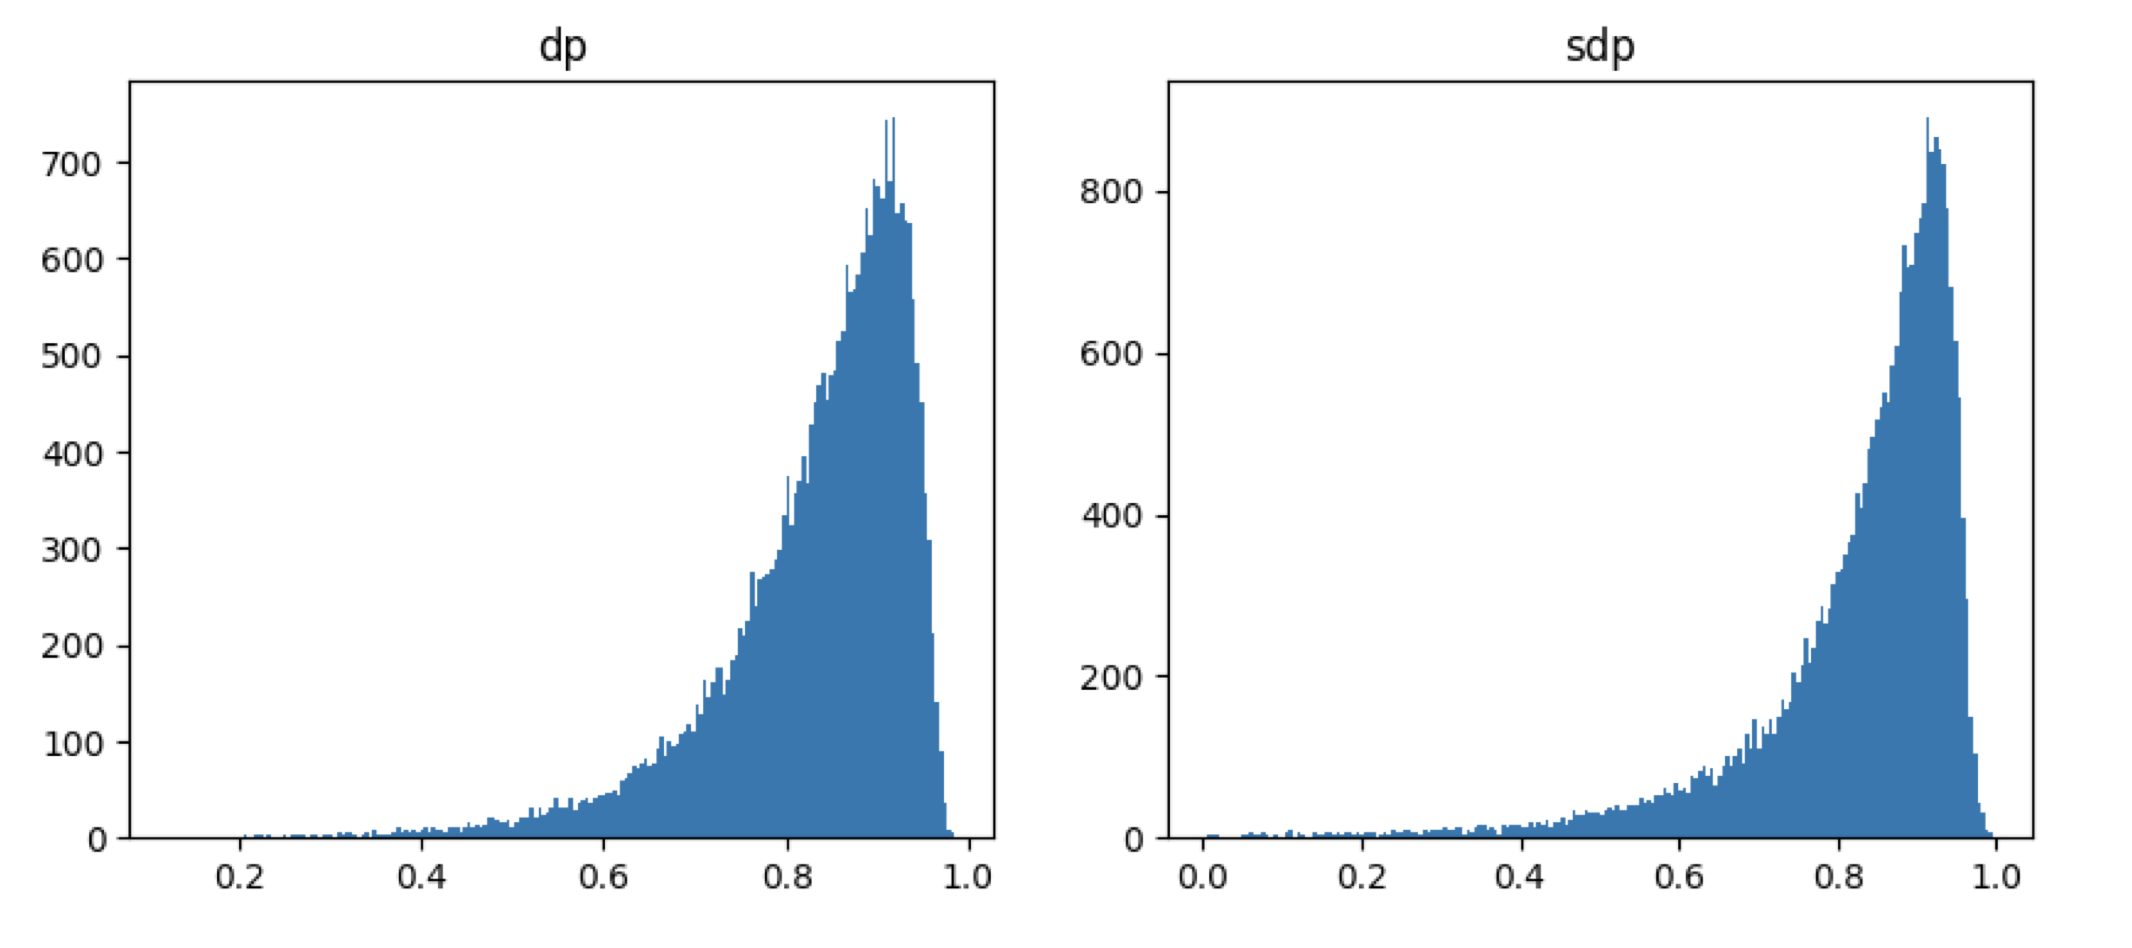
\includegraphics[width=.825\hsize,height=.15\hsize]{neims-hist}
\end{tabular}
\end{frame}

\begin{frame}
{RASSP -- výsledky}
\begin{itemize}
\item[$+$] Vyšší přesnost
\item[$+$] Vysoké rozlišení, větší kontrola nad izotopy
\item[$-$] Citelně pomalejší
\item[$-$] Strašidelný (neudržovatelný) rozsáhlý kód 
\begin{itemize}
\item mix TF, PyTorch (1.x), C++/Python, spousta mrtvého kódu,\\ akcelerovaně jen na AMD (WTF?), obskurní multithreading, \dots
\end{itemize}
\item[$-$] Omezení na 8 typů atomů, 4096 podformulí (!!)
\begin{itemize}
\item redukuje NIST z 300k na 140k
\item rozšířit lze, rychle rostou nároky na paměť GPU (80 GB je málo)
\end{itemize}
\end{itemize}
\end{frame}

\begin{frame}
{Bonusové implementace}
\begin{itemize}
\item Grafová konvoluční síť, grafová síť s~\emph{attention}, grafový transformer
\item Všechny použity v~kombinaci s~NEIMS (MLP), v~architektuře nahrazují fingerprinty
\item Postupně rostoucí přesnost 

\bigskip
\begin{tabular}{|l|r|r|r|r|}
\hline
& DP & SDP & inference (h/28k) & train (h/113k) \\
\hline
NEIMS &
$0.832 \pm 0.108 $&
$0.828 \pm 0.136 $&
$0.10 $&
$4.50 $\\
GCN &
$0.850 \pm 0.114 $&
$0.847 \pm 0.155 $&
$0.12 $&
$5.50 $\\
GAT &
$0.858 \pm 0.110 $&
$0.859 \pm 0.147 $&
$0.15 $&
$12.00$ \\
Transformer &
$0.860 \pm 0.110 $&
$0.865 \pm 0.141 $&
$0.20 $&
$15.00$ \\
RASSP &
$0.886 \pm 0.119 $&
$0.882 \pm 0.158 $&
\color{gray}{$120$} (*)&
$200.00 $\\
\hline
\end{tabular}

\end{itemize}
\end{frame}

\begin{frame}
{Shrnutí}
\begin{itemize}
\item Publikované implementace jsou vesměs použitelné, výsledky lze přiměřeně reprodukovat
\item Získali jsme solidní znalost problematiky a odpovídající intuici
\item Implementace jsou nasaditelné pro konkrétní úlohy na centru Recetox
\item Máme nástroj ke generování dat pro ,,cestu zpátky`` (navazující příspěvek)
\end{itemize}
\end{frame}

\end{document}
